\documentclass[rmp,10pt,onecolumn,fleqn,notitlepage]{revtex4-1}

\usepackage{graphicx}
\usepackage{color}
\usepackage{latexsym,amsmath}
\usepackage{physics}
\usepackage{tabularx}
\usepackage{float}
\usepackage{siunitx}
\usepackage{amssymb}

% Listing packages
\usepackage{xcolor}
\usepackage{listings}
\usepackage{framed}
\usepackage{inconsolata} % To change the listing font

% URL package and setting
\definecolor{linkcolor}{rgb}{0,0,0.65} %hyperlink
\usepackage[pdftex,colorlinks=true, pdfstartview=FitV, linkcolor= linkcolor, citecolor= linkcolor, urlcolor= linkcolor, hyperindex=true,hyperfigures=true]{hyperref} %hyperlink%

\usepackage{fancyhdr} % To change page setting

% PAGE SETTING
\pagestyle{fancyplain}
\fancyhf{}
\fancyfoot[R]{\thepage}
\fancyfoot[L]{\today}
\fancyhead[L]{\textbf{Week 5 Report, Quantum Information and Computing (2020)}}
\fancyhead[R]{\textbf{Alice Pagano}}
\renewcommand{\headrulewidth}{0.1pt}
\renewcommand{\footrulewidth}{0.1pt}

% LISTING SETTINGS
\definecolor{cadmiumred}{rgb}{0.89, 0.0, 0.13}
\definecolor{codegray}{rgb}{0.5,0.5,0.5}
\definecolor{commentcolour}{rgb}{0.43,0.63,0.65}
\definecolor{darkgreen}{rgb}{0.0, 0.5, 0.0}

\lstdefinestyle{Fortran}{language=Fortran,
    backgroundcolor=\color{white},
    commentstyle=\color{commentcolour},
    keywordstyle=\bfseries\color{cadmiumred},
    numberstyle=\tiny\color{codegray},
    stringstyle=\color{darkgreen},
    basicstyle=\ttfamily\footnotesize,
    breakatwhitespace=false,
    breaklines=true,
    captionpos=b,
    keepspaces=true,
    numbers=left,
    numbersep=5pt,
    showspaces=false,
    showstringspaces=false,
    showtabs=false,
    tabsize=2,
    frame=single,
    framexleftmargin=11pt,
    %rulecolor=\color{cadmiumred}
}
%\lstset{style=Fortran}

\lstdefinestyle{Gnuplot}{
    backgroundcolor=\color{white},
    commentstyle=\color{commentcolour},
    basicstyle=\ttfamily\footnotesize,
    breakatwhitespace=false,
    breaklines=true,
    captionpos=b,
    keepspaces=true,
    showspaces=false,
    showstringspaces=false,
    showtabs=false,
    tabsize=2
}

\lstdefinestyle{Python}{language=Python,
    backgroundcolor=\color{white},
    commentstyle=\color{commentcolour},
    keywordstyle=\color{darkgreen},
    numberstyle=\tiny\color{codegray},
    stringstyle=\color{cadmiumred},
    basicstyle=\ttfamily\footnotesize,
    breakatwhitespace=false,
    breaklines=true,
    captionpos=b,
    keepspaces=true,
    numbers=left,
    numbersep=5pt,
    showspaces=false,
    showstringspaces=false,
    showtabs=false,
    tabsize=2,
    frame=single,
    framexleftmargin=11pt
}

% BIBLIOGRAPHY FILE AND SETTING
\begin{filecontents*}{\jobname.bib}
    @article{cite1,
      title={Error handling in Fortran 2003},
      author={Koen Poppe and Ronald Cools and Bart Vandewoestyne},
      journal={ACM Sigplan Fortran Forum},
      year={2012},
      volume={31},
      pages={7-19}
    }
\end{filecontents*}

\bibliographystyle{aipnum4-1}
\setcitestyle{numbers,square}








\begin{document}



\title{Week 5: Eigenproblem and Random Matrix Theory}
\author{Alice Pagano}
\date{\today}

\begin{abstract}
In this Report, we compute the distribution of normalized spacing between eigenvalues for a random hermitian matrix and a diagonal matrix. We fit the obtained distribution with a curve and we analyze their behavior as a function of different level constants used to compute the local average between eigenvalues.
\end{abstract}

\maketitle


\section{Theory}
A \textbf{diagonal matrix} is a matrix in which the entries outside the main diagonal are all zero;  the term usually refers to square matrices.

A \textbf{hermitian matrix} is a complex square matrix that is equal to its own conjugate transpose, that is:
\begin{equation}
  A \text{ Hermitian } \iff a_{ij} = \bar{a}_{ji}
\end{equation}
The finite-dimensional \textbf{spectral theorem} says that any Hermitian matrix can be diagonalized by a unitary matrix, and that the resulting diagonal matrix has only real entries. This implies that all \emph{eigenvalues} of a Hermitian matrix $A$ with dimension $n$ are \emph{real}, and that $A$ has $n$ \emph{linearly independent eigenvectors}.
Moreover, a convenient way to store in a computer an Hermitian matrix is by exploiting the so called \textbf{packed storage matrix}. It is a more compact way than an $n$-by-$n$ rectangular array by exploiting the special structure of the hermitian matrix: the lower triangle of $A$ is stored column-by-column in vector $AP$.


Let us diagonalize matrix $A$ and let us suppose to obtain $n$ eigenvalues \( \lambda _i \) stored in \emph{crescent order}. The \textbf{normalized spacing} between eigenvalues \( s_i \) is defined as:
\begin{equation}
    s_i = \frac{\Delta \lambda _i }{ \expval{\Delta \lambda _i} } \qquad \text{with}  \quad
  \Delta \lambda _i = \lambda _{i+1} - \lambda _i
  \label{eq:si}
\end{equation}
where the average spacing $\expval{\Delta \lambda _i}$ can be computed \emph{globally} (by averaging over all spacing \( \Delta \lambda _i \)) or \emph{locally}, i.e. over a different number of levels around \( \lambda _i \) (as \( n/100 \), \( n/50 \), \( n/10 \) and so on).


The \textbf{distribution} \( P(s) \) of normalized spacing \( s_i \) for a random Hermitian matrix, or for a random diagonal matrix, can be fitted with the following function:
\begin{equation}
  P(s) = a s^{\alpha } \exp(- b s^{\beta })
  \label{eq:distribution}
\end{equation}
Moreover, for each type of matrix we can compute the average \( \expval{r}  \) of:
\begin{equation}
  r_i = \frac{\min(\Delta \lambda _i, \Delta \lambda _{i+1})}{\max( \Delta \lambda _i, \Delta \lambda _{i+1})}
  \label{eq:ri}
\end{equation}
and compare the results for the two different cases.
% include bibliography
%\bibliography{\jobname}

\section{Code Development}

In order to study both hermitian and diagonal matrix of size \( n \), we develop one different program for each type of matrix. In particular, the two programs differ only for the matrix initialization, as:
\begin{itemize}
\item in “hermitian.f90” we define a complex random vector \texttt{AP} of size \( np = n (n+1)/2 \) which is initialized trough Lapack \texttt{SUBROUTINE} {\bfseries\texttt{zlarnv}} and which stores the lower triangle of \texttt{A}. Then, we unpack the vector \texttt{AP} to matrix \texttt{A}.

\begin{minipage}[t]{0.4\linewidth}%\vspace{0pt}
\begin{lstlisting}[style=Fortran]
! initialize random vector AP
call zlarnv(3,iseed,np,AP)

! unpacking matrix AP to A
do jj=1,n
    k = jj*(jj-1)/2
    A(1:jj,jj) = AP(1+k:jj+k)
    A(jj,1:jj-1) = conjg(AP(1+k:jj-1+k))
end do\end{lstlisting}
\end{minipage}


\item in “diagonal.f90” we define a real random vector \texttt{AP} of size \( n \) which is initialized trough Lapack \texttt{SUBROUTINE} {\bfseries\texttt{dlarnv}} and which stores the diagonal of \texttt{A}. Then, we unpack the vector \texttt{AP} to matrix \texttt{A}.

\begin{minipage}[t]{0.4\linewidth}%\vspace{0pt}
\begin{lstlisting}[style=Fortran]
! initialize random vector AP
call dlarnv(3,iseed,np,AP)

! unpacking matrix AP to A
do ii=1,n
    A(ii,ii) = cmplx(AP(ii),0)
end do\end{lstlisting}
\end{minipage}

\end{itemize}
Then, the structure of the two main programs is exactly the same. In order, when each program is executed:
\begin{enumerate}
\item the dimension of the matrix \texttt{n}, the number of bins for the histogram \texttt{nbins}, the number of times the matrix is computed \texttt{ntime} and the fixed \texttt{level} for the local average are taken in input;
\item then, for \texttt{ntime} times:

    \begin{enumerate}
    \item matrix \texttt{A} is random initialized with a \textbf{normal distribution} in \( (0,1) \) (as explained before);

    \item eigenvalues are computed and ordered in \emph{ascending order} using Lapack \texttt{SUBROUTINE} {\bfseries\texttt{zheev}};

    \item eigenvalues spacing are computed (Eq. \eqref{eq:si}) and stored in array \texttt{delta$\_$eig} of dimension \texttt{n-1};

    \item then, we compute the global average \texttt{aver$\_$delta$\_$eig} and the corresponding global normalized spacing \texttt{norm$\_$delta$\_$eig}. We add the normalized spacing into an array \texttt{si} of dimension \texttt{ntime(n-1)} which stores the results of global normalized spacing for each execution;

    \item after that, we compute the local average of spacing array \texttt{local$\_$aver$\_$delta$\_$eig} of dimension \texttt{n-1}. In particular, let us consider a generic eigenvalue \( \lambda _i \), to compute its local average, we average over the eigenvalue itself, \texttt{level} eigenvalues at its left and \texttt{level} eigenvalues at its right, for a total of \( 2  \texttt{level} + 1 \) elements.
    We have to pay attention to the eigenvalues at the extremes, which do not have enough elements at their left or right. To solve that problem, for each eigenvalue whose index is lower than \texttt{level}, or higher than \texttt{n-1-level}, we assume their average to be equal to the average of the first, or the last, \texttt{level+1} elements. Then, we compute the normalized spacing \texttt{local$\_$norm$\_$delta$\_$eig} and we add them into an array \texttt{local$\_$si} of dimension \texttt{ntime(n-1)} which stores the results of local normalized spacing for each execution;


    \begin{minipage}[t]{0.85\linewidth}%\vspace{0pt}
    \begin{lstlisting}[style=Fortran]
! compute local average spacing
aver_sx = (eig(2*level+1+1)-eig(1)) / (2*level+1)
aver_dx = (eig(n)-eig(n-2*level-1)) / (2*level+1)

do ii=1,n-1
    if (ii <= level) then
        local_aver_delta_eig(ii) = aver_sx
    else if (ii > n-1-level) then
        local_aver_delta_eig(ii) = aver_dx
    else
        local_aver_delta_eig(ii) = (eig(ii+level+1)-eig(ii-level)) / (2*level+1)
    endif
end do\end{lstlisting}
    \end{minipage}

    \item at the end, we compute \( \expval{r}  \) (Eq. \eqref{eq:ri}) and we write the result for each execution into a file;
    \end{enumerate}

\item at the end, we compute the probability function for both the global and local normalized spacing by using \texttt{SUBROUTINE} {\bfseries\texttt{create$\_$histogram}} of the user-defined \texttt{MODULE} {\bfseries\texttt{histogram}}. This subroutine, which will explain in more details later, takes as input the entries of the histogram, the fixed number of bins \texttt{nbins} and a specified range \( [\min,\max] \) which we fix to \( [0,5] \). The bin centers and the normalized entries are printed into a file.

\end{enumerate}

In the file “histogram.f90”, we define \texttt{MODULE} {\bfseries\texttt{histogram}} which contains the \texttt{SUBROUTINE} {\bfseries\texttt{create$\_$histogram}}. In particular, when the last subroutine is called, the following operations occurs in order:
\begin{enumerate}
\item we fix the bin width \texttt{dx} (equal for all the bins) to the range \texttt{(max-min)} divided by the number of bins \texttt{nbins};
\item we compute bin centers \texttt{bin$\_$centers} and left bin edges \texttt{bin$\_$edges} (plus the most right edge);
\item we fill bins with events and we store the number of events for each bin in the array \texttt{hist};
\item we normalize the histogram by dividing the entries of \texttt{hist} by the total histogram area \texttt{tot$\_$area}, obtaining the array \texttt{norm$\_$hist};
\item the obtained results are printed into a file whose name is dictaed by \texttt{file$\_$name} variable in a folder called \texttt{folder$\_$name}.
\end{enumerate}

\begin{minipage}[t]{0.85\linewidth}%\vspace{0pt}
\begin{lstlisting}[style=Fortran]
subroutine create_histogram(events,n_bins,min,max,file_name,folder_name)
    ...
    real(8), dimension(n_bins) :: bin_centers
    real(8), dimension(n_bins+1) :: bin_edges
    real(8), dimension(n_bins) :: hist, norm_hist
    ...
    ! compute bin width
    dx = (max-min) / n_bins

    ! compute bin centers
    do ii=1,n_bins
        bin_centers(ii) = min + dx/2 + (ii-1)*dx
    end do

    ! compute left bin edges (plus the most right edge)
    do ii=1,n_bins+1
        bin_edges(ii) = min + (ii-1)*dx
    end do

    ! compute histogram
    do ii=1,n_bins
        ! fill bins with events
        do jj=1,size(events,1)
            if (events(jj)>=bin_edges(ii) .and. events(jj)<=bin_edges(ii+1)) then
                hist(ii) = hist(ii) + 1
            end if
        end do
    end do

    ! compute total histogram area
    tot_area = size(events) * dx

    ! compute normalized histogram
    do ii=1,n_bins
        norm_hist(ii) = hist(ii)/tot_area
    end do

    ...

    ! write data into file
    do ii=1,n_bins
        write(file,*) bin_edges(ii), bin_centers(ii), hist(ii), norm_hist(ii)
    end do

end subroutine create_histogram\end{lstlisting}
\end{minipage}

After that, we develop a Python script “script.py” in which:
\begin{itemize}
\item we fix the matrix size \texttt{N}, the number of times \texttt{Ntime} the matrix is computed, the number of bins for the histogram \texttt{Nbins} and a list of \texttt{level} we want to study;

\item then, for each \texttt{lev} in \texttt{level}, we execute “hermitian” and “diagonal” executables.

\item finally, for both diagonal and hermitian matrices, we call a Gnuplot script “plot$\_$hist.p” which produces a plot of normalized spacing distribution for global and local average (for the different levels) with the corresponding fit (Eq. \eqref{eq:distribution}).
\end{itemize}

\begin{minipage}[t]{0.85\linewidth}%\vspace{0pt}
\begin{lstlisting}[style=Python]
executable = ['hermitian','diagonal']

# Compile programs
make_command = ["make","all"]
make_proc = subprocess.run(make_command)

# Define variables
N      = 5000
Ntime  = 10
Nbins  = 100

level = [10,50,100,250,1000]

for lev in level:
    for exe in executable:
        print("Type  : ", exe)
        print("N     : ", N)
        print("Nbins : ", Nbins)
        print("Level : ", lev)
        print("Ntime : ", Ntime,'\n')

        result = subprocess.run(['./'+exe,str(N),str(Nbins),str(Ntime),str(lev)])

# Plot histogram
for exe in executable:
    result = subprocess.run(['gnuplot','-e',"file_name='"+exe,'plot_hist.p'])\end{lstlisting}
\end{minipage}

\section{Results}

In order to have enough statistics for the normalized spacing distribution, we choose a large matrix size of \texttt{N=5000} and we compute it \texttt{Ntime=10} times. In this way, we obtain \( 50000 \) events for the histogram for which we fix \texttt{Nbins=100}. The plots obtained are illustrated in Fig. \ref{fig:results}.
We note that normalized spacing \( s_i \), for both hermitian and diagonal matrices, distributes accordingly to Eq. \eqref{eq:distribution}, but with fit parameters quite different.
This result is in accordance with the theory since both of them belong to the same ensamble of symmetric matrices.
For hermitian matrices, we note that there is only a slightly difference between the distribution for different levels. Instead, for diagonal matrices the difference is more evident.

\begin{figure}[h!]
\begin{minipage}[c]{0.49\linewidth}
\centering
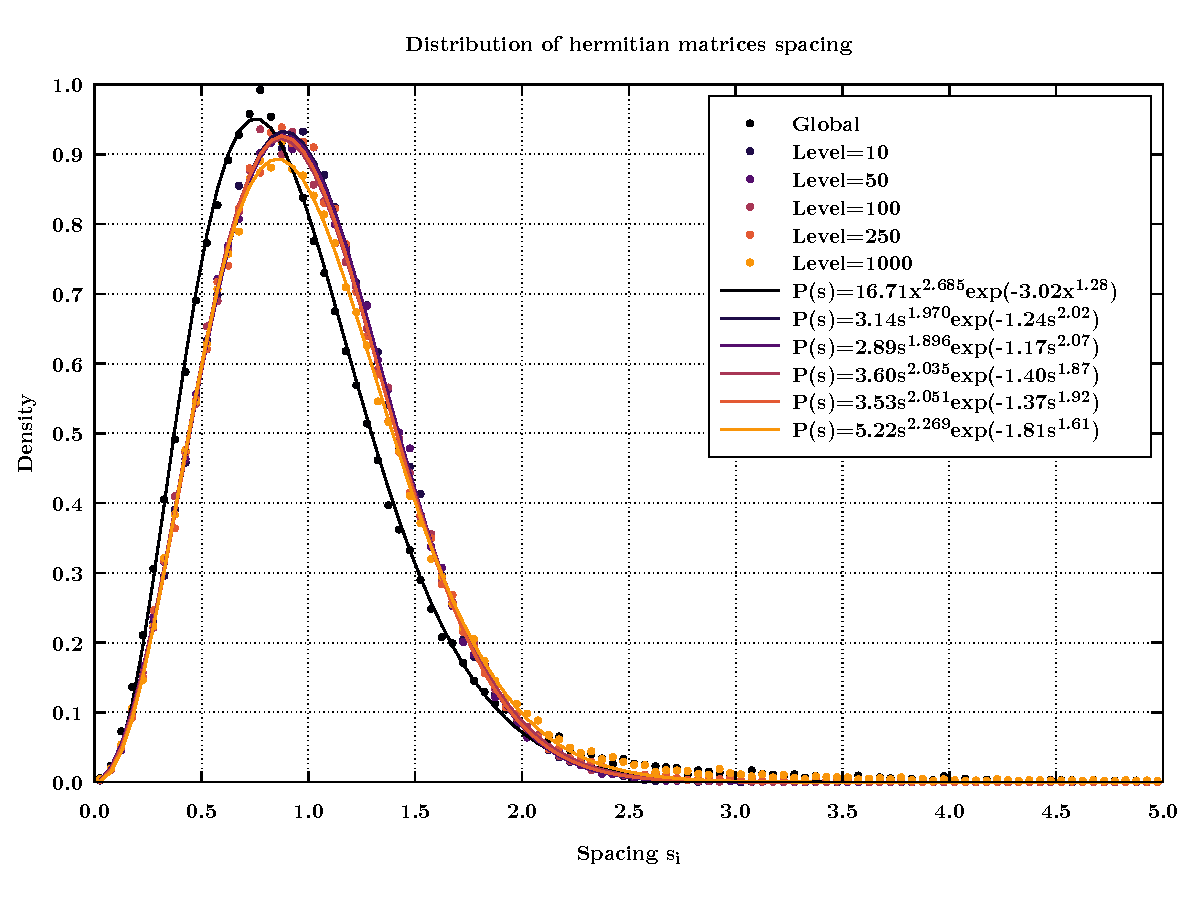
\includegraphics[width=1\textwidth]{image/hist_hermitian-local.pdf}
\end{minipage}
\begin{minipage}[]{0.5\linewidth}
\centering
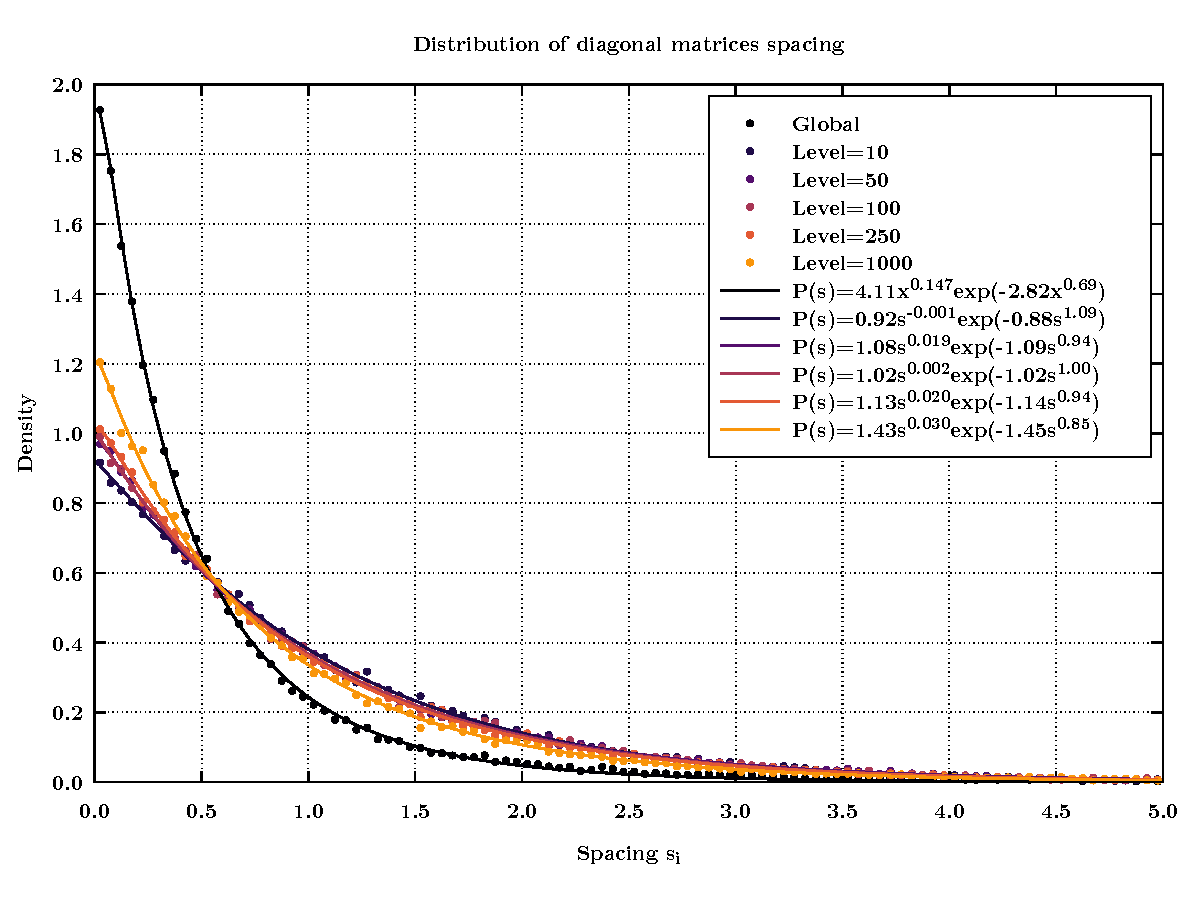
\includegraphics[width=1\textwidth]{image/hist_diagonal-local.pdf}
\end{minipage}
\caption{\label{fig:results} Plots of normalized spacing distribution for global and local average (with different levels choosen). \textbf{Left:} case of hermitian matrices. \textbf{Right:} case of diagonal matrices. }
\end{figure}

Moreover, we compute the \( \expval{r}  \) for the different matrices. The results are:
\begin{equation}
  \expval{r}_{\text{hermitian}} = 0.600 \pm 0.004, \qquad \expval{r}_{\text{diagonal}} =  0.387 \pm 0.003
\end{equation}


\section{Self-evaluation}
In a further development of the code, it would be interesting to study the behavior of the spacing distribution for matrices which are random initialized with different distribution (not only normal one) to see if their distribution is in accordance with Eq. \eqref{eq:distribution}. Moreover, it would be interesting to study other types of random matrices to explore in more details random matrix theory.






\end{document}
